% `advanced_example.tex', an advanced example employing the AIAA class
% plus other third-party LaTeX packages.
%
% For a bare-bones usage, see `template.tex'.
%
% Typical processing for PostScript (PS) output:
%
%  latex advanced_example
%  bibtex advanced_example  (bibliography)
%  makeindex -s nomencl.ist -o advanced_example.gls advanced_example.glo
%                            (nomenclature)
%  latex advanced_example   (repeat as needed to resolve references)
%
%  xdvi advanced_example    (onscreen draft display)
%  dvips advanced_example   (postscript)
%  gv advanced_example.ps   (onscreen display)
%  lpr advanced_example.ps  (hardcopy)
%
% With the above, only Encapsulated PostScript (EPS) images can be used.
%
% Typical processing for Portable Document Format (PDF) output:
%
%  pdflatex advanced_example
%  bibtex advanced_example    (bibliography)
%  makeindex -s nomencl.ist -o advanced_example.gls advanced_example.glo
%                              (nomenclature)
%  pdflatex advanced_example  (repeat as needed to resolve references)
%
%  acroread advanced_example.pdf  (onscreen display)
%
% If you have EPS figures, you will need to use the epstopdf script
% to convert them to PDF because PDF is a limmited subset of EPS.
% pdflatex accepts a variety of other image formats such as JPG, TIFF,
% PNG, and so forth -- check the documentation for your version.
%
% If you do *not* specify suffixes when using the graphicx package's
% \includegraphics command, latex and pdflatex will automatically select
% the appropriate figure format from those available.  This allows you
% to produce PS and PDF output from the same LaTeX source file.
%
% To generate a large format (e.g., 11"x17") PostScript copy for editing
% purposes, use
%
%  dvips -x 1467 -O -0.65in,0.85in -t tabloid advanced_example
%
% For further details and support, read the Users Manual, aiaa.pdf.

\documentclass[]{aiaa-tc}% insert '[draft]' option to show overfull boxes

 \usepackage{varioref}%  smart page, figure, table, and equation referencing
 \usepackage{wrapfig}%   wrap figures/tables in text (i.e., Di Vinci style)
 \usepackage{threeparttable}% tables with footnotes
 \usepackage{dcolumn}%   decimal-aligned tabular math columns
  \newcolumntype{d}{D{.}{.}{-1}}
 \usepackage{nomencl}%   nomenclature generation via makeindex
  \makeglossary
 \usepackage{amssymb,amsmath}
 \usepackage{subfigure}% subcaptions for subfigures
 \usepackage{subfigmat}% matrices of similar subfigures, aka small mulitples
 \usepackage{fancyvrb}%  extended verbatim environments
 \fvset{fontsize=\footnotesize,xleftmargin=2em}
 \usepackage{lettrine}%  dropped capital letter at beginning of paragraph
%  \usepackage[dvips]{dropping}% alternative dropped capital package
 \usepackage[colorlinks]{hyperref}%  hyperlinks [must be loaded after dropping]
 \usepackage{float}
 \usepackage{longtable,booktabs,tabularx}
 \restylefloat{table}
 \usepackage{graphicx}
 \usepackage{caption}
 \usepackage{multicol}
 \usepackage[labelfont=bf]{caption}

 \title{Solar-Electric and Gas Powered, Long-Endurance UAV Sizing via Geometric Programming}

 \author{
  Michael Burton \thanks{Master's Candidate, Aeronautical and Astronautical Engineering, 77 Mass Ave, Cambridge MA, 02139, AIAA Student.}
  \ and Warren Hoburg\thanks{Professor, Aeronautical and Astronautical Engineering, 77 Mass Ave, Cambridge MA, 02139, AIAA Member.}\\
  {\normalsize\itshape
   Massachusetts Institute of Technology, Cambridge, 02139, USA}\\
 }

 % Data used by 'handcarry' option
 \AIAApapernumber{YEAR-NUMBER}
 \AIAAconference{Conference Name, Date, and Location}
 \AIAAcopyright{\AIAAcopyrightD{YEAR}}

 % Define commands to assure consistent treatment throughout document
 \newcommand{\eqnref}[1]{(\ref{#1})}
 \newcommand{\class}[1]{\texttt{#1}}
 \newcommand{\package}[1]{\texttt{#1}}
 \newcommand{\file}[1]{\texttt{#1}}
 \newcommand{\BibTeX}{\textsc{Bib}\TeX}

\begin{document}

\maketitle

\begin{abstract}
    Using geometric programming, a comparison of solar-electric and gas powered, long-endurance aircraft is accomplished.
    Long-endurance aircraft present a complicated systems engineering problem because of the multifaceted interaction of various requirements, such as endurance, velocity and coverage footprint.
    Geometric programming, a form of convex optimization, can reliably solve problems with thousands of variables in seconds and is used as an optimization tool to evaluate the design trade offs between architectures and requirements.
    Using this approach, a gas powered and a solar-electric powered aircraft were considered.  
    The results show that long-endurance, gas powered aircraft are generally more robust to higher wind speeds than solar-powered aircraft.  
    However, gas powered aircraft are limited in their endurance by the amount of fuel that they can carry. 
    While solar-electric powered aircraft can theoretically fly for months, they are operationally limited by limited sunlight during the winter and wind speeds at higher latitudes.
    Using geometric programming, a detailed trade study between gas-powered and solar-powered aircraft is performed to discover which architecture is best suited to meet a given set of requirements, and what is the optimum size and endurance of that platform.
\end{abstract}

\section*{Nomenclature}

\begin{multicols}{2}
\small

\begin{tabbing}
  XXXXXXX \= \kill% this line sets tab stop
$A$ \> wing aspect ratio \\
$BSFC$ \> brake specific fuel consumption [lb/hr/hp] \\
$c$ \> wing chord [m] \\
$C_D$ \> drag coefficient \\
$C_{d_0}$ \> non-wing drag coefficient \\
$c_{d_p}$ \> wing profile drag coefficient \\
$C_L$ \> lift coefficient \\
$\Delta y$ \> wing section length [m] \\
$\Delta W$ \> wing section weight [N] \\
$DOY$ \> day of the year \\
$e$ \> Oswald efficiency factor \\
$E$ \> Young's Modulus [Pa] \\
$E_{\text{battery}}$ \> energy stored in battery [J] \\
$(E/S)_{\text{sun}}$ \> total solar energy available [Whr/m$^2$] \\
$f_{\text{solar}}$ \> planform area fraction covered in solar cells \\
$f_{\text{structural}}$ \> fractional structural weight\\
$g$ \> gravitational constant [m/s$^2$] \\
$h$ \> flight altitude [ft] \\
$h_{\text{cap}}$ \> spar cap separation [m] \\
$I$ \> moment of inertia [m$^4$] \\
$K_q$ \> wing loading constant [N/m$^2$] \\
$L$ \> atmospheric lapse rate [K/m] \\
$\dot{m}_{\text{fuel}}$ \> fuel flow rate [kg/s] \\
$M$ \> wing bending moment [Nm] \\
$MTOW$ \> max take-off weight [N] \\
$n$ \> number of wing segments \\
$N$ \> number of flight segments \\
$N_{max}$ \> load factor\\
$P_{0}$ \> magnitude of available solar power [W/m$^2$] \\
$P_{\text{avionics}}$ \> avionics power [hp] \\
$P_{\text{oper}}$ \> aircraft operating power [hp] \\
$P_{\text{shaft}}$ \> engine shaft power [hp] \\
$P_{\text{sun}}$ \> useable solar power [W/m$^2$] \\
$P_{\text{sun surface}}$ \> power emitted at the sun's surface [W/m$^2$] \\
$r_0$ \> average distance from earth to sun \\
$R$ \> aircraft range [nmi] \\
$R_{\text{earth orbit}}$ \> distance from earth to sun \\
$R_{\text{spec}}$ \> specific gas constant [J/k/K] \\
$R_{\text{sun}}$ \> radius of the sun \\
$q$ \> distributed wing loading [N/m] \\
$Re$ \> Reynolds number \\
$S$ \> wing planform area [m$^2$]\\
$\mathcal{S}$ \> shear forces [N] \\
$S_{\text{solar}}$ \> solar cell area [m$^2$]\\
$t$ \> flight time [days] \\
$t_{\text{cap}}$ \> spar cap thickness [m] \\
$t_{\text{day}}$ \> hours of daylight [hr] \\
$t_{\text{night}}$ \> hours of darkness [hr] \\
$t_{\text{sun rise}}$ \> time of sun rise [hr] \\
$t_{\text{sun set}}$ \> time of sun set [hr] \\
$T$ \> aircraft thrust [N] \\
$T_{\text{atm}}$ \> air temperature at flight altitude [K] \\
$T_{\text{sl}}$ \> air temperature at sea level [K] \\
$V$ \> true airspeed [m/s] \\
$V_{min}$ \>  minimum true airspeed [m/s] \\
$w$ \> wing deflection [m] \\
$W$ \> aircraft weight [N] \\
$W_{\text{ave}}$ \> average weight over a flight segment [N] \\
$W_{\text{battery}}$ \> battery weight [N] \\
$w_{\text{cap}}$ \> spar cap width [m] \\
$W_{\text{final}}$ \> final aircraft weight [N] \\
$W_{\text{fuel}}$ \> fuel weight [N] \\
$W_{\text{initial}}$ \> initial aircraft weight [N] \\
$w_{max}$ \> maximum deflection limit [m] \\
$W_{\text{payload}}$ \> payload weight [N] \\
$W_{\text{solar}}$ \> solar cell weight [N] \\
$W_{\text{structural}}$ \> structural weight [N] \\
$z_{bre}$ \> Breguet Range helper variable \\
$\Delta$ \> solar declination angle \\
$\Delta h_{\text{fuel}}$ \> heat of combustion [J/kg] \\
$\eta_{\text{charge}}$ \> battery charging efficiency \\
$\eta_{\text{discharge}}$ \> battery discharging efficiency \\
$\eta_{prop}$ \> propulsive efficiency \\
$\eta_{\text{solar}}$ \> solar cell efficiency \\
$\mu$ \> air viscosity [kg/m/s] \\
$\phi$ \> latitude \\
$\rho$ \> air density [kg/m$^3$] \\
$\rho_{\text{carbon fiber}}$ \> density of carbon fiber [kg/m$^3$] \\
$\rho_{\text{solar}}$ \> solar cell density [kg/m$^2$] \\
$\sigma_{\text{carbon fiber}}$ \> maximum carbon fiber stress [Pa] \\
$\tau_t$ \> wing thickness to chord ratio \\
$\tau_w$ \> cap spar width to chord ratio \\
$\theta$ \> angle normal to surface \\
$\Theta$ \> bending deflection angle 
 \end{tabbing}

\end{multicols}
% \printglossary% creates nomenclature section produced by MakeIndex

\section{Introduction}

The design problem of a long-endurance, station-keeping aircraft is considered.
Solar electric and gas powered architectures are proposed as solutions to this problem.
Because sizing long-endurance aircraft is so multifaceted and the interaction between aerodynamics, structural weight, energy and other disciplines is so intertwined, a systematic and rapid approach is needed to explore this design space.
Geometric programming, a form of convex optimization, is chosen as a means of evalulating the design space because of its ability to solve optimization problems involving thousands of variables in seconds.  

The driving condition that sizes solar-electric powered aircraft is operationality or the ability to operate at multiple locations and during all seasons.  
To achieve a feasible design, solar-electric powered aircraft must carry enouh solar cells and batteries required to fly during the day while storing enough energy to fly through the night. 
If this condition can be achieved during the winter solstice, when the solar flux is at a minimum, then it can theoretically fly for months at a time. 
This becomes more difficult to achieve at higher latitudes as the solar flux durin the winter solstice decreases.  
Additionally, to station keep the aircraft must fly faster than the local wind speeds.  
Wind speeds are a function of latitude, altitude, and season and tend to increase at higher latitudes and during winter months. 
Therefore, a key sizing study of solar-electric powered aircraft is the effect of latitude on aircraft size.  
Figure~\ref{f:bvslatsolar} shows that in order to fly at higher latitudes during the winter a larger aircraft is required. 

\begin{figure}[H]
	\begin{center}
	\includegraphics[width=0.6\textwidth]{bvslatsolar.pdf}
    \caption{ \textbf{ Trade study showing how aircraft size increases with latitude.  }}
	\label{f:bvslatsolar}
	\end{center}
\end{figure}

The key driving requirement for gas-powered aircraft is endurance.  
As gas-powered aircraft are endurance limited by the amount of fuel that they can carry, longer endurance requires more fuel and hence a larger aircraft.  
Becuase gas-powered aircraft are not affected by the solar flux, their station-keeping ability at different latitude only depends on wind speed. 
Therefore, if a gas-powered aircraft can fly at the latitude with the worst wind speed in can theortically fly anywhere else in the world.  
The key sizing study for the gas-powered airctaft is how weight increases for longer endurance. (Figure~\ref{f:mtowvsendurance}) 

\begin{figure}[H]
	\begin{center}
	\includegraphics[width=0.6\textwidth]{mtowvsendurance.pdf}
    \caption{ \textbf{ Trade study showing how aircraft weight increases with endurance.  }}
	\label{f:mtowvsendurance}
	\end{center}
\end{figure}

To capture the interaction of all of these parameters and requirements and produce the resutls presented, a geometric programming optimization model is built for both the gas and solar-electric powered, long-endurance aircraft.  
Equations governing the underlying physics of aerodynamic performance, solar energy collection and storage, and fuel burn are written in a geometric programming form which can then be solved as an optimization problem.
Then by changing the design parameters, such as endurance, latitude, and percentile wind speeds, multiple solutions can be rapidly generated to observe how the aircraft size and weight is affected by different requirements. 

Using this methodology, trade offs are observed between different aircraft configurations, power sources, and requirements.  
The results show that gas-powered aircraft can generally be built lighter and can fly faster and can therefore fly at higher latitudes and in higher percentile wind speeds.  
Solar-powered aircraft have greater endurance but are limited operationally by their ability to reach higher speeds.  
This optimization methodology can quantify the difference in weight and endurance between and gas and solar-electric powered aircraft for the same set of requirements. 
Similar trade offs are calculated for other requirements and performance metrics to determine under what conditions which platform is best suited to meet a set of requirements.

\section{Geometric Programming\cite{gp}}

Geometric programs (GPs) are a mathematical optimization problem characterized by the convexity of the objective and constraint functions. GPs have the form

\begin{align} 
\label{e:gpform}
\text{minimize } f_0(\bold{x}) & \nonumber \\
\text{subject to  } f_i(\bold{x}) &\leq 1, i=1,...,m \\
g_i (\bold{x}) &= 1, i = 1,...,p \nonumber 
\end{align}

where the functions $f_i$ must be \emph{monomial} functions and the functions $g_i$ must be \emph{posynomial} functions. \emph{Monomials} and \emph{posynomials} have the forms

\begin{align}
 \label{e:mon}
g(\bold{x}) &= c x_1^{a_1} x_2^{a_2} \dotsm x_n^{a_n} , \\
\label{e:pos}
f(\bold{x}) &= \displaystyle\sum_{k=1}^K c_k x_1^{a_{1_k}} x_2^{a_{2_k}} \dotsm x_n^{a_{n_k}}.
\end{align}

The properties of a geometric program allow solution algorithms to guarantee convergence to a global optimum, provided that there exists a feasible solution to the set of constraint functions.  
Additionally, geometric programs can be solved rapidly with existing algorithms.  
Using state of the art, standard interior-point algorithms, GPs with 1,000 variables and 10,000 constraints converge to a solution in tens of seconds.\cite{gp}  
To solve an aircraft design problem, all physical models are expressed as constraints on the GP.\cite{hoburgthesis} \\

\section{Aircraft Sizing Models}

To evaluate the size and performance of both gas and solar-electric powered aircraft basic physics models are used.  
Environmental models describing the effect of altitude, latitude and season on wind speeds, air density, and solar insolation and aircraft models governing the performance, aerodynamics and weight breakdown are used in the optimization model.
Equations from these models are then expressed in a GP-compatible form to enable their use in the optimization. 
Understanding the models that are used in a GP is important because the solution to a GP is only as accurate as the models that are used to construct the program.  
To obtain higher fidelity results from the optimization, higher fidelity models can be implemented. 

\subsection{Station Keeping}

Long-endurance, station keeping aircraft are generally required to operate at specific latitudes, altitudes, and percentile wind speeds. Both wind speeds and atmospheric quantities depend on the station keeping requirements. 

\subsubsection{Wind Speeds}

To station keep, an aircraft must fly faster than the wind speed.  
Therefore, the aircraft speed is constrained for both the gas and solar-electric powered cases,

\begin{equation}
    \label{e:availreq}
    V \geq V_{wind}.
\end{equation}

The wind speed at a station is a function of latitude, altitude, season or day of the year, and percentile wind speed,

\begin{equation}
    \label{e:windspeed}
    V_{wind} = f(\phi, h, DOY, \text{Percentile Wind Speed}).
    \end{equation}

Wind speed data was collected from the ERA Interim atmospheric datasets for the years 2005-2015.\cite{wind} 
It is assumed that the wind speeds can be approximated by using wind data across all longitudes. 

Because wind speeds vary by season, an analysis was done of how wind speeds varyfrom month to month. (Figure~\ref{f:windvsmonth}) Becasue the constraining case for solar-electric powered aircraft is the winter solstice and because the wind speeds are highest during the winter months only the wind speeds from December will be used for all aircraft sizing and performance analysis. 

\begin{figure}[H]
	\begin{center}
	\includegraphics[width=0.6\textwidth]{windvsmonth.pdf}
    \caption{ \textbf{ Variation of wind speed by month at 45 degrees latitude at altitudes of 15,000 ft, 50,000 ft and 60,000 ft.  Left bound, right bound and middle lines represent 85th, 95th, and 90th percentile winds. }}
	\label{f:windvsmonth}
	\end{center}
\end{figure}

Figure~\ref{f:latvswind} shows how the wind speed varies with latitude in the Northern Hemisphere. 
The left bound on the graphs represent the 85 percentile winds.  The right bound represents the 95 percentile winds and the middle line represents the 90 percentile winds. 
Because the gas-powered aircraft is assumed to have a naturally aspirated engine, it will tend to fly around 15,000 ft.  
The solar-electric powered aircraft will operate around 60,000 ft to avoid cloud coverage.  
Variations of wind speed with latitude are shown for altitudes at both 15,000 ft at and 60,000 ft.  \\

\begin{figure}[H]
	\begin{center}
	\includegraphics[width=0.6\textwidth]{latvswind.pdf}
    \caption{ \textbf{ Variation of wind speed with latitude at altitudes of 15,000 ft, 50,000 ft and 60,000 ft.  Left bound, right bound and middle lines represent 85th, 95th, and 90th percentile winds. Wind data includes winds during December for the year 2005-2015.}}
	\label{f:latvswind}
	\end{center}
\end{figure}

Wind speeds also vary signifactly with altitude. (Figure~\ref{f:altvswind.pdf})
The high winds around 30,000-40,000 ft makes it difficult for both solar-electric and gas powered long-endurance aircraft to fly in that range of altitudes.  
Solar-electric powered aircraft, that do not have aspirated engines, fly around 60,000 ft take advantage of lower wind speeds and limited cloud coverage.
Gas powered aircraft with aispirated engines can have difficulty operating at 60,000 ft and generally perform better in the lower wind speeds below 25,000 ft.

\begin{figure}[H]
	\begin{center}
	\includegraphics[width=0.6\textwidth]{altvswind.pdf}
    \caption{ \textbf{ Variation of wind speed with altitude at latitudes of 30, 35, and 45 degrees.  Left bound, right bound and middle lines represent 85th, 95th, and 90th percentile winds. Wind data includes winds during December for the year 2005-2015.}}
	\label{f:altvswind}
	\end{center}
\end{figure}

Because both air density and wind speed vary with altitude, the optimium altitude for the solar-electric powered aircraft at a given latitude is not clear. 
Additionally, the local minimum around 60,000 ft feet suggests that altitude should be a variable chosen by the optimizer. 
To achieve this, the data fitting technique described by Hoburg\cite{fitting}, was used to find functions relating wind speed to air density at a given latitude.  
Air density was chosen as the dependent variable to eliminate altitude as the intermediate variable betweeen air density and wind speed relation. 
An example contraint of wind speed and air density at the 35 degree latitude is written out in Equation~\ref{e:windfit35},


\begin{align}
    \label{e:windfit35}
    \left(\frac{V_{wind}}{V_{ref}}\right)^{7.213} &>= 2918\rho^{7.587}p_{wind}^{9.37} + 1.58e^{-10}\rho^{-6.074}p_{wind}^{60.421} + 4.05e^{-16}\rho^{-9.879}p_{wind}^{13.204} + 1048\rho^{6.33}p_{wind}^{46.232}
\end{align}

where $V_{ref} = 100$ [m/s] and $p_{wind}$ is the percentile wind speed. The comparison of the fitted equation to the actual data is presented in Figure~\ref{f:windfitl35}. 

\begin{figure}[H]
	\begin{center}
	\includegraphics[width=0.6\textwidth]{windfitl35.pdf}
    \caption{ \textbf{ Comparison of a fitted equation of wind speed to air density and percentile wind speed~\eqref{e:windfit35}. The RMS error for this function and data set is 0.043. Wind speed data includes December wind speeds from 2005-2015 at the 35th degree latitude. }}
	\label{f:windfitl35}
	\end{center}
\end{figure}

Similars equations to~\eqref{e:windfit35} were generated for wind speed data from latitudes 20-60 degrees in the Northern Hemisphere (See Appendix A).  The equations are valid within 45,000-80,000 ft to within 5\% of the actual data. 

Operationally, aircraft, such as the solar-electric powered aircarft, will fly within a band of latitudes (i.e. $\pm$45 degrees latitude).  
To achieve a band of latitude operationality the aircraft must be able to fly at every latitude between the upper and lower bounds.  
For this reason, latitude was not included as a varible in the fitted equation.  
Instead to optimize an aircraft for 35 degrees latitude means that the there are 35 seperate wind constraints that must be satisfied, one for each latitude.
Because wind speeds are low and solar flux is higher below 20 degrees latitude no constraints for latitudes below 20 degrees are actually included in the optimization. 

For the gas powered aircraft, the altitude is not optimized.  
Gas-powered aircraft, which are naturally aspirated will be less effecient at higher altitudes.  
Additionally, wind speeds increase nearly linearly up to 30,000 ft.  
Therefore, the altitude for gas-powered aircraft is determined as a requirement of the payload and the minimum altitude necessary for the payload to be effective. 

\subsubsection{Atmospheric Quantities}

For the solar aircraft air density is being optimized and the operating altitude is computed after the fact using Equations~\ref{e:tropopress} and~\ref{e:tropoalt} \cite{isaatm} that apply to the tropopause, 

\begin{align}
    \label{e:tropopress}
    p &= \rho RT_{11} \\
    \label{e:tropoalt}
    h &= 11000 - \frac{RT_{11}}{g}\frac{p}{p_{11}} \text{[m]} 
\end{align}

According to Sutherland's law\cite{fluiddyhandbook}, viscosity varies with temperature.  Because temperature is assumed constant above 11,000 meters\cite{isaatm}, viscosity is assumed to be constant, $\mu=1.42e^{-5}$.

Because altitude is a requirement for the gas powered aircraft, density is precomputed prior to solving the optimization using similar atmospheric equations for the troposphere,\cite{isaatm} 

\begin{align}
    \label{e:Talt}
    T_{\text{atm}} = T_{\text{sl}} - Lh \\
    \label{e:rhot}
    \rho = \frac{T_{\text{sl}}T_{\text{atm}}^{\left( \frac{g}{R_{\text{spec}}L} -1 \right)}}{R T_{\text{sl}}^{\frac{g}{R_{\text{spec}}L}}}.
\end{align}

Air viscosity is also computer prior so solving and is assumed to vary according to Sutherland's law, 

\begin{equation}
    \label{e:sutherland}
    \mu = \mu_0 \frac{T_0 + C}{T+C} \left( \frac{T}{T_0} \right)^{\frac{3}{2}}
\end{equation}

where $\mu_0 = 1.827e^{-5}$ [Ns/m$^2$], $T_0 = 291.15$ [K], and $C = 120$ [K].

\subsection{Solar-Electric Power}

The driving equations for the solar-electric powered aircraft are determined by the energy required to fly throughout the day while charging the batteries enough to last through the night.  
Equations~\ref{e:solarreq} and~\ref{e:solarbatt} capture the solar requirement by enforcing that the total solar energy harvested by the solar cells during the day must be greater than the energy used to operate the aircraft during the day while charging enough batteries to fly during the night. 
Under these assumptions, if the aircraft can fly for one day and one night, then it could theoretically fly for many days under similar circumstances. 

    \begin{align}
        \label{e:solarreq}
        (E/S)_{\text{sun}} \eta_{\text{solar}} S_{\text{solar}} &\geq P_{\text{oper}}t_{\text{day}} + E_{\text{battery}}/\eta_{\text{charge}} \\
        \label{e:solarbatt}
        E_{\text{battery}} &\geq P_{\text{oper}}t_{\text{night}}/\eta_{\text{discharge}}
    \end{align}
    
    It is assumed that the charge and discharge efficiencies are constant, $\eta_{charge} = \eta_{discharge} = 0.98$. It is also assumed that the solar cell efficiency is constant, $\eta_{solar} = 0.3$. A battery with a energy density of, $h_{batt} = 350$, is selected for the solar-powered aircraft. 

    To enforce these constraints, two variables were created: $P_{\text{oper}}$ and $S_{\text{solar}}$. 
    $P_{\text{oper}}$ is defined as the average power required to operate the aircaft. \eqref{e:solarpoper} 
    $S_{\text{solar}}$ is defined as the amount of area on the aircraft covered by solar cells. \eqref{e:solarssolar}

    \begin{align}
        \label{e:solarpoper}
        P_{\text{oper}} &\geq P_{\text{shaft}} + P_{\text{avionics}} \\
        \label{e:solarssolar}
        S_{\text{solar}} &\leq f_{\text{solar}}S
    \end{align}

    For the purposes of this design study, it is assumed that the solar cells are only placed on the wing and that the total solar cell area is limited to some fraction of the wing planform area to account for control surfaces, leading edge, and other accessories.  \\

    Because solar aircraft requirements are typically given in terms if latitude and yearly availability it is useful to express the total available solar energy per unit area per day as a function of latitude, $\phi$, and the day of the year, $DOY$, 
    
    \begin{equation}
        \label{e:solarfunc}
        (E/S)_{\text{sun}} = f(\phi, DOY).
    \end{equation}


    For simplicity, energy and power will refer to energy and power per unit area throughout the rest of this section. (i.e. $(E/S) = E$) The total available solar energy per day is an integral of the available solar power during the course of the day.

    \begin{equation}
        \label{e:solares}
        E_{\text{sun}} = \int_{t_{sunrise}}^{t_{sunset}} P_{\text{sun}} dt
    \end{equation}

    Figure~\ref{f:lat45} shows a sample distribution of the available solar power during the spring equinox at 45 degrees latitude. 
    
\begin{figure}[H]
	\begin{center}
	\includegraphics[width=0.6\textwidth]{lat45.pdf}
    \caption{ \textbf{ The available solar power per unit area during the spring equinox in the Northern Hemisphere at $\phi=45^{\circ}$.  The area under this curve is the total energy available per unit area for the entire day.} }
	\label{f:lat45}
	\end{center}
\end{figure}

The shape of this curve is governed by the angle, $\theta$, between the normal to the flat surface, or aircraft wing, and the sun beam.\cite{solar}

\begin{equation}
    \label{e:solarp}
    P_{\text{sun}} = P_0 \cos{\theta}
\end{equation}

The angle, $\theta$ depends on the time of day, latitude, and declination angle,\cite{solar}

    \begin{equation}
        \label{e:solartheta}
        \cos{\theta} = \sin{\Delta} \sin{\phi} + \cos{\Delta} \cos{\phi} \cos{2\pi t/24},
    \end{equation}

    where $\Delta$ is the declination angle at solar noon, $\phi$ is the latitude, and $t$ is the time of day.\cite{solar}  The declination angle, $\Delta$,can be found using the relation\cite{solar} 

    \begin{align}
        \label{e:solardelta}
        \Delta = &0.006918 - 0.399912 \cos{\beta} + 0.070257\sin{\beta} - 0.006758\cos{2\beta} + \nonumber \\
        & 0.000907\sin{2\beta} - 0.002697\cos{3\beta} + 0.00148\sin{3\beta},
    \end{align}

    where, $\beta = 2\pi (DOY-1)/365$.  \\

    The time of day and the time of night can be calculated using a derivation Equation~\ref{e:solartheta}, \cite{solar}

    \begin{align}
        \label{e:solartday}
        \cos{(\pi t_{\text{sun rise}}/12)} &= -\tan{\Delta} \tan{\phi} \\
        \label{e:solarsunrise}
        t_{\text{sun rise}} &= -t_{\text{sun set}} \\
        \label{e:solartday2}
        t_{\text{day}} &= 2t_{\text{sun rise}} \\
        \label{e:solartnight}
        t_{\text{night}} &= 24 - t_{\text{day}}
    \end{align}

    where noon is $t=0$. Both $t_{\text{day}}$ and $t_{\text{night}}$ affect the battery size as defined in Equations~\ref{e:solarreq} and~\ref{e:solarbatt}. \\

    The solar power available assuming no inclination angle, $P_0$, is found using the eccentricity of the earth's orbit, 

    \begin{align}
        \label{e:solarp0}
        P_0 & = P_{\text{sun surface}} \frac{R_{\text{sun}}^2}{R_{\text{earth orbit}}^2}, \\
        \label{e:solareo}
        R_{\text{earth orbit}} & = r_0 \left[ 1 + 0.017 \sin{\left( 2\pi \frac{DOY-93}{365}\right)} \right],
    \end{align}
    
    where 

    \[ \begin{array}{lcl}
        P_{\text{sun surface}} & : & \text{Power emitted at the sun's surface} \\
        R_{\text{sun}} & : & \text{Radius of the sun} \\
        R_{\text{earth orbit}} & : & \text{Distance from earth to sun} \\
        r_0 & : & \text{Average distance from earth to sun} \\
        0.017 & : & \text{Eccentricity of earth-sun orbit}.
    \end{array} \]

    Using a trapezoidal integration of Equation~\ref{e:solares}, the total available solar energy per unit area can be obtained for a given latitude and day of the year. Because only Equations~\ref{e:solarreq}-\ref{e:solarssolar} are GP compatible, the total solar energy per unit area per day, the length of the day and the length of the night is calculated from the latitude and the day of the year prior to an optimization solve.

\subsection{Breguet Range}

A key sizing equation for a long endurance gas powered aircraft is the Breguet Range equation.  
For GP-compatibility and to optimize endurance, not range, a variation of the Breguet Range equation is used, 

\begin{equation}
    \label{e:breguetendurance}
    t = \frac{W_{\text{ave}}}{P_{\text{shaft}}BSFCg} \ln{\left( \frac{W_{\text{initial}}}{W_{\text{final}}}\right)}.
\end{equation}

The derivation begins with the differential form of Breguet Range,\cite{br2}

\begin{equation}
    \label{e:breguetdiff}
    -\frac{dW}{dt} = g\dot{m}_{\text{fuel}}.
\end{equation}

Using the definition of $BSFC$

\begin{equation}
    \label{e:brBSFC}
    BSFC = \frac{\dot{m}_{\text{fuel}}}{P_{\text{shaft}}},
\end{equation}

Equation~\ref{e:breguetdiff} can be written as

\begin{equation}
    \label{e:brdiff2}
    -dW = g P_{\text{shaft}} BSFC dt.
\end{equation}

It is assumed that $BSFC$ and the power to weight ratio, $(P_{\text{shaft}}/W)$, are constant during the considered flight segment. 
A constant power to weight ratio assumes constant velocity and constant lift coefficient.\cite{br2}
Dividing by $W$,

\begin{equation}
    \label{e:brdiff2}
    -\frac{dW}{W} = \frac{g P_{\text{shaft}}BSFC }{W} dt,
\end{equation}

and integrating, the Breguet Range equation can be expressed as

\begin{equation}
    \label{e:be1}
    \ln{\left( \frac{W_{\text{initial}}}{W_{\text{final}}} \right)} = \frac{gP_{\text{shaft}}BSFC}{W_{\text{ave}}} t,
\end{equation}

where $W_{\text{ave}}$ is the average weight of the aircraft during the flight segment.  $W_{\text{ave}}$ is assumed to be the geometric mean, defined as

\begin{equation}
    \label{e:gpmean}
    W_{\text{ave}} = \sqrt{W_{\text{initial}}W_{\text{final}}}.
\end{equation}

    To make Equation~\ref{e:be1} GP compatible, a Taylor expansion of the exponentiated right hand side is used,\cite{hoburgthesis}

\begin{align}
    \label{e:brzbre}
    z_{bre} &\geq \frac{P_{\text{shaft}}t BSFC g}{W}\\
    \label{e:brtaylor}
    \frac{W_{\text{fuel}}}{W_{final}} &\geq z_{bre} + \frac{z_{bre}^2}{2} + \frac{z_{bre}^3}{6} + \frac{z_{bre}^4}{24} + \dots
\end{align}

    Equations~\ref{e:brzbre} and~\ref{e:brtaylor} are monomial and posynmial respectively and therefore GP compatible. \\
    
    For long-endurance aircraft, missions can last days, causing the power to weight ratio $(P_{\text{shaft}}/W)$ to vary significantly during the course of the flight.  Equations~\ref{e:brzbre},~\ref{e:brtaylor}, and~\ref{e:slfweight} can be discretized for more accurate results.

\begin{align}
    \label{e:slfweightd}
    \sqrt{W_i W_{i+1}} &= \frac{1}{2} \rho_i V_i^2 C_{L_i} S \\
    \label{e:brzbred}
    z_{bre_i} &\geq \frac{P_{shaft_i}t_i BSFC g}{\sqrt{W_i W_{i+1}}}\\
    \label{e:brtaylord}
    \frac{W_{fuel_i}}{W_{i+1}} &\geq z_{bre_i} + \frac{z_{bre_i}^2}{2} + \frac{z_{bre_i}^3}{6} + \frac{z_{bre_i}^3}{24} 
    \end{align}

    For evaluation of long-endurance, gas-powered aircraft a discretization of $N=5$ is used. Additionally, it is assumed that the break specific fuel consumption is constant, $BSFC = 0.6$ [lb/hr/hp].

\subsection{Steady Level Flight}

Both the gas and solar powered aircraft are assumed to be in steady level flight.  The balance of the main forces of lift, drag, weight and thrust are modeled as

\begin{align}
    \label{e:slfthrust}
    T &\geq \frac{1}{2} \rho V^2 C_D S\\
    \label{e:slfweight}
    W &= \frac{1}{2} \rho V^2 C_L S . 
\end{align}

The shaft power produced by the engine or motor and can expressed as  

\begin{equation}
    \label{e:slfpower}
    P_{\text{shaft}} = \frac{TV}{\eta_{prop}}
    \end{equation}

    where the propulsive efficiency is assumed to be a constant, $\eta_{prop} = 0.75$. Equations~\ref{e:slfthrust},~\ref{e:slfweight}, and~\ref{e:slfpower} are all monomials and therefore GP-compatible.

\subsection{Aerodynamics}

The aircraft aerodynamics is modeled as a drag build up of wing profile drag, induced drag, and non-wing drag coefficients, 

\begin{equation}
    \label{e:aerodragb}
    C_D \geq C_{d_0} + c_{d_p} + \frac{C_L}{\pi e A}.
    \end{equation}

where the Oswald efficiency factor is assumed to be constant, $e=0.9$. 
The non-wing drag coefficient, $C_{d_0}$, is estimated as a constant.  
For the gas powered aircraft, $C_{d_0} = 0.005$.  
For the solar-electic powered aircraft, $C_{d_0} = 0.002$.  
It is assumed that gas powered aircraft will have a higher non-wing drag coefficient that a solar powered aircraft because a gasoline energy source will require a fuselage with a larger frontal area than a battery energy source.\cite{raymer}
    
    Because fuel has a higher volume to energy ratio than batteries, it is assumed that the gas powered aircraft will have some sort of fuselage to hold the fuel while the solar-electric powere aircraft will store the batteries in the wings and have no fuselage.  This difference in configuration accounts for the higher non-wing drag coefficient of the gas powered aircraft.  
    
    To estimate the wing profile drag, a posynomial fit is made of the drag polar of the \emph{JH01} airfoil. (See Appendix) 
    Drag polars were produced using XFOIL at various Reynolds and the data was then fit to a posynomial equation using techniques described in Hoburg.\cite{fitting}
    The XFOIL drag polar data is compared to the posynomial fit in figure~\ref{f:JH01polar}.

    \begin{align}
        \label{e:aerodragprof}
        c_{d_p}^{3.72} &\geq  0.0247C_L^{2.49}Re^{-1.11} + 2.03e^{-7}C_L^{12.7}Re^{-0.338} + 6.35e^{10}C_L^{-0.243}Re^{-3.43} + 6.49e^{-6}C_L^{-1.9}Re^{-0.681}\\
        Re &= \frac{\rho V S/b}{\mu}
    \end{align}

\begin{figure}[H]
	\begin{center}
	\includegraphics[width=0.6\textwidth]{JH01polar.pdf}
    \caption{ \textbf{ The posynomial fit (Equation~\ref{e:aerodragprof}) of the \emph{JH01} airfoil drag polar is represented as a solid line.  The open circles are the calculated drag polars from XFOIL. The maximum residual error, as defined in Hoburg\cite{fitting}, is 0.00489.} }
	\label{f:JH01polar}
	\end{center}
\end{figure}


As a preliminary sizing study the aspect ratio is assumed to be a constant, $A = 30$.  A more detailed sizing study with a wing structural model, discussed later, will allow the aspect ratio to be a free variable. 

\subsection{Weight Breakdown}

The weight of each component of both the gas and solar platforms is summed to constrain the max take off weight.  
The structural weight comprises the weight of the wing, fuselage, horizontal and vertical stabilizer, and engine. 
The weight breakdown for the gas powered aircraft is a summation of the structural weight, the total fuel weight, and the payload weight. 

\begin{align}
    \label{e:weightmtow}
    MTOW &\geq W_{\text{structural}}  + W_{\text{payload}} + W_{\text{fuel}} \\
\end{align}

A similiar weight breakdown is done for the solar-electric powered aircraft, 

\begin{align}
    \label{e:weightsmtow}
    MTOW &\geq W_{\text{structural}} + W_{\text{payload}} + W_{\text{solar}} + W_{\text{battery}} \\
    W_{\text{solar}} &\geq \rho_{solar} S_{solar} g \\
    W_{\text{battery}} &\geq \frac{E_{\text{battery}}}{h_{\text{battery}}} g
\end{align}


% \subsection{Comparison to Existing Platforms}
% 
% By comparing the results of the optimization model to existing gas-powered, long-endurance platforms confidence is gained in the validity of the models.  
% Known pramaters from the Orion, Predator, Global Hawk, Hermes and Penguin (Table~\ref{t:existingparams}) aircraft are inputed to the optimization model.  
% A comparison of the results from the optimization model and the actual aircraft endurance is summarized in table~\ref{t:existingplatforms} and figure~\ref{f:vehiclecomp}. The model is then solved by maximizing endurance.
% 
% \begin{longtable}{lcccc}
%     \caption{Known Parameters of Exisiting Long Endurance Aircraft}\\
%      \toprule
%      \toprule
%      \label{t:existingparams}
%      Aircraft & MTOW [lbf] & Cruise Speed [m/s] & Altitude [ft] & Payload Weight [lbf]\\
%      \midrule
%      Orion\cite{orion}      & 11,200 & 34  & 15,000 & 1,500\\
%      Predator\cite{predator}   & 2,250  & 70  & 25,000 & 450\\
%      Hermes\cite{hermes}     & 2,600  & 70  & 30,000 & 771\\
%      Global Hawk\cite{globalhawk}& 32,250 & 160 & 50,000 & 3,000\\
%      Penguin\cite{penguin}    & 47    & 22   & 10,000 & 22\\
%      \bottomrule
%  \end{longtable}
% 
%  Additionally, the parameters in table~\ref{t:compparams} are set as constants for each comparison optimization solve. 
% 
% \begin{longtable}{ll}
%     \caption{Fixed Optimization Parameters} \\
%      \toprule
%      \toprule
%      Variable &  Value \\
%      \midrule
%      $\eta_{prop}$        & 0.65   \\
%      $A$                 & 25     \\
%      $f_{\text{structural}}$     & 0.35   \\
%      $BSFC$ [lb/hp/hr]    & 0.6    \\
%      \bottomrule
%      \label{t:compparams}
%  \end{longtable}
% 
%  \begin{figure}[H]
%  \begin{subfigmatrix}{2}% number of columns
%      \subfigure[MTOW Comparison\label{f:mtowvehiclecomp}]{\includegraphics{mtowvehiclecomp.pdf}}
%      \subfigure[Span Comparison\label{f:bvehiclecomp}]{\includegraphics{bvehiclecomp.pdf}}
%  \end{subfigmatrix}
%  \caption{ \textbf{Comparison of optimization results to existing platforms.  Each aircraft's unique parameters from table~\ref{t:existingparams} are set as fixed constants in the optimization model.} }
%  \label{f:vehiclecomp}
% \end{figure}
%  
% \begin{longtable}{lcccc}
% \caption{Optimization Results Comparison} \\
% \label{t:existingplatforms} \\
%      \toprule
%      \toprule
%      Aircraft & Actual Endurance [days] & Predicted Endurance [days] & Actual Span [ft] & Predicted Span [ft]\\
%      \midrule
%      Orion      & 5 & 4.4   & 132 & 146.8\\
%      Predator   & 1  & 1.7  & 55 & 39.0 \\
%      Hermes     & 1.5 & 1.2 & 50  & 47.27\\
%      Global Hawk& 1.5 & 1.0 & 131 & 100.6\\
%      Penguin    & 1 & 1.6   & 10.8  & 15.14\\
%      \bottomrule
%  \end{longtable}
% 
% 
% Because of limited information about these aircraft the optimization predictions are not exact. However, it does validate the proposition that the geometric programming optimzation model is useful for approximating the size and performance of long-endurance aircraft because the results of the optimization are within the same order of manitude as the existing aircarft. 

\section{Long-endurance Aircraft Trade Space}

One way to analyze the trade space is to determine the structural weight of the aircraft as some percentage of the total aircraft weight, 

\begin{equation}
    \label{e:structualfraction}
    W_{structural} \geq f_{structural}MTOW.
\end{equation}

where the structural fraction is assumed to be, $f_{structural} = 0.35$. Using this assumption and models described in section III, a comparison of the long-endurance trade space is achieved by comparing solar-electric and gas powered aircraft for different parameters. 

% \begin{longtable}{llll}
% \caption{Fixed Optimization Parameters} \\
% \toprule
% \toprule
% \multicolumn{2}{c}{Gas Powered} & \multicolumn{2}{c}{Solar Powered}\\
% \midrule
% Latitude [deg]       & 45     & Latitude [deg]       & 30 \\
% Altitude [ft]        & 16,000 & Altitude [ft]        & 50,000        \\
% Payload Weight [lbf] & 10     & Payload Weight [lbf] & 10            \\
% $\eta_{prop}$        & 0.75   & $\eta_{prop}$        & 0.75          \\
% $A$                 & 25     & $A$                 & 25              \\
% $f_{\text{structural}}$ & 0.35   & $f_{\text{structural}}$ & 0.35    \\
% $c_{d_0}$            & 0.005  & $c_{d_0}$            & 0.002         \\ 
% $BSFC$               & 0.6    & $\eta_{\text{charge}}$      & 0.98   \\
% Endurance [days]     & 8      & $\eta_{\text{discharge}}$   & 0.98   \\
%                      &        & $h_{\text{battery}}$ [Whr/kg]  & 350 \\
%                      &        & $\rho_{\text{solar}}$ [kg/m$^2$] & 0.3 \\
%                      &        & Day of the Year      & 355 (Dec 21st)\\
% \bottomrule
% \label{t:gassolarparams}
%  \end{longtable}


\subsection{Sizing for Different Latitude Bands}

An analysis of the max take off weight required to operate at different latitudes reveals that is it is more difficult for solar-electric powered aircraft to operate at higher wind speeds than it is for gas powered aircraft.
This analysis is achieved by minimizing the max take off weight in both the gas and solar-electric powered optimization models at different latitudes. 
For this study, the gas-powered aircraft is constrained to fly for 8 days. 

\begin{figure}[H]
 \begin{subfigmatrix}{2}% number of columns
     \subfigure[Gas Powered\label{f:mtowvslatgas}]{\includegraphics{mtowvslatgas.pdf}}
     \subfigure[Solar-Electric Powered\label{f:mtowvslatsolar}]{\includegraphics{mtowvslatsolar.pdf}}
 \end{subfigmatrix}
 \caption{\textbf{ Trade study of max take off weight and latitude. Plots show required maximum take off weight required to operate between a band of latitudes.   A comparison of the solar and gas powered latitude analysis shows that gas powered aircraft are more robust to operating in higher wind speeds. Results are valid for the models described in section III.}}
 \label{f:latvsmtowtrade}
\end{figure}

One way to interpret Figure~\ref{f:latvsmtowtrade} is that a solar-powered aircraft weighing ... is able to opeate between 0 and 35 degrees latitude in 90 percentile wind, assuming that the models and parameters described in section II are accurate.  
This analysis shows that gas powered architectures are more robust to operating in more locations than solar-electric powered aircraft.  
Figure~\ref{f:mtowvslatgas} levels off around 35 degrees latitude because that is the latitude of highest wind speeds at 15,000 ft.  
Thus, if the gas powered aircraft can fly at 35 degrees latitude it can fly in band of latitudes greater than 0 to 35.  
On the other hand, solar-electric powered aircraft design becomes less feasible at higher latitudes because after 40 degrees latitude wind speeds are higher and solar flux is lower. 

\subsection{Gas Powered Endurance}

While, gas powered aircraft may be more robust to high wind speeds, solar-electric powered aircraft can achieve higher endurance. 
The gas powered optimization model was set to minize max take off weight for different endurance requirements to understand what endurance limits are possible. 

\begin{figure}[H]
	\begin{center}
	\includegraphics[width=0.6\textwidth]{solargasmtow.pdf}
    \caption{ \textbf{ Trade study between endurance and max take off weight for a gas powered archicture. }}
	\label{f:solargasmtow}
	\end{center}
\end{figure}

For a gas-powered archicture, achieving endurances above 10 days requires an aircraft that is likely infeasible to build.  Solar-electric powered aircraft, however, can theoretically fly indefinitely. 

\subsection{Solar-electric Powered Trade Space Exploration}

For a broader picture of the design space the solar optimization is solved multiple times, producing a set of contour plots for various battery energy densities, structural fraction weights, altitudes, and availabilities.  (Figure~\ref{f:solarcontours}) 
The matrix contour plot map is a useful reference tool designed to give understanding to key trade offs in the solar-electric powered aircraft sizing problem.

 \begin{figure}[H]
 \begin{subfigmatrix}{3}% number of columns
  \subfigure[40th Latitude, 80\% Wind Speed]{\includegraphics{bcontourl40a80.pdf}}
  \subfigure[40th Latitude, 85\% Wind Speed]{\includegraphics{bcontourl40a85.pdf}}
  \subfigure[40th Latitude, 90\% Wind Speed]{\includegraphics{bcontourl40a90.pdf}}
  \subfigure[35th Latitude, 80\% Wind Speed]{\includegraphics{bcontourl35a80.pdf}}
  \subfigure[35th Latitude, 85\% Wind Speed]{\includegraphics{bcontourl35a85.pdf}}
  \subfigure[35th Latitude, 90\% Wind Speed]{\includegraphics{bcontourl35a90.pdf}}
  \subfigure[30th Latitude, 80\% Wind Speed]{\includegraphics{bcontourl30a80.pdf}}
  \subfigure[30th Latitude, 85\% Wind Speed]{\includegraphics{bcontourl30a85.pdf}}
  \subfigure[30th Latitude, 90\% Wind Speed]{\includegraphics{bcontourl30a90.pdf}}
 \end{subfigmatrix}
 \caption{ \textbf{Matrix of contour plots of battery energy density and structural weight fraction vs wing span for solar-electric powered aircraft. Each point on the graph corresponds to a unique design.} }
 \label{f:solarcontours}
\end{figure}

\section{Detailed Models}

To improve the fidelity of the optimization, higher fidelity models can be implemented.  
A spar and structural wing model are added to both the gas and solar-electric powered optimization models.  
Additionally, an empennage model is added to account for the additional weight and drag of horizontal and vertical tails and a tail boom.  
These models, similar those described in section III, are a set of constraints derived from governing first principles put in a GP-compatible form. 
This results in a more comprehensive and detailed optimization model for aircraft sizing.   \\

\subsection{Wing Spar Model}

A simple approach to modeling a wing spar is to assume that the wing is a beam under bending loads caused by the lifting distribution along the wing and the weight of the aircraft. 
A conservative approach to calculating the size of the spar is to assume that the spar carries all of the bending loads.  

For the gas powered aircraft it is assumed that all of the fuel is carried. 
Therefore the key spar sizing case is a standard wing bending acting under both lifting and gravitational forces, 

\begin{equation}
    \label{e:wloading}
    q(y) = L'(y) - Ngm'(y)
\end{equation}

where $q$ is the spanwise distributed load. 
The wing loading distribution, $q$, can be approximated by scaling of the local chord,\cite{bending}

\begin{equation}
    \label{e:wingloading}
    q(y) \approx K_q c(y) 
\end{equation}

where $y$ is the distance from the root wing location. The loading constant $K_q$\cite{bending} is defined as

\begin{equation}
    \label{e:kq}
    K_q = \frac{N_{max}W_{cent}}{S}
\end{equation}

where $W_{cent}$ is the sum of distributed loads acting at the center of the aircraft and the safety load factor is, $N=5$. The local chord for a constant tapered wing\cite{bending} is defined as 

\begin{equation}
    \label{e:localchord}
    c(y) = \frac{S_{wing}}{b} \frac{2}{1+\lambda} \left( 1 + (\lambda - 1) \frac{2y}{b} \right)
\end{equation}

where the taper ratio is $\lambda=0.5$. 
For the solar-electic powered aircraft it is assumed that the batteries are located inside the wings.  
Therefore, it is assumed that the key sizing case for the solar-electric aircraft spar is a gust load that varies arcross the span.  
The distributed load across the span is assumed to be 

\begin{equation}
    \label{e:gustdist}
    \bar{q} = c_{l_{\alpha}} \alpha_{gust} \frac{1}{C_L} \left( 1 + \frac{W_{cent}}{W_{wing}} \right)
\end{equation}

where the lifting slope coefficient is, $c_{l_{\alpha}}=2\pi$, and $\alpha_{gust}$ is the local angle of attack caused by the gust. The local angle of attack is approximated by 

\begin{equation}
    \label{e:gustalpha}
    \alpha_{gust} = \tan^{-1}\left(\frac{V_{gust}}{V} \right).
\end{equation}

Because the $\arctan$ function is not GP compatible a monomial approximation was calculating using techniques described by Hoburg\cite{fitting},

\begin{equation}
    \label{e:arctan}
    \alpha_{gust} = 0.855922 \left(\frac{V_{gust}}{V} \right)^{0.934041}.
\end{equation}

This approximation is graphically shown in Figure~\ref{f:arctanfit}.  Even though Equation~\ref{e:arctan} is only valid up to gust speed to aircraft speed ratios of, $\frac{V_{gust}}{V} = 0.7$, ...

\begin{figure}[H]
	\begin{center}
	\includegraphics[width=0.6\textwidth]{arctanfit.pdf}
    \caption{ \textbf{ Comparison of monomial approximation of $f(x) = \arctan{x}$ to real function, $x \in [0,1]$. (RMS error = 0.044) }}
	\label{f:gustvschord}
	\end{center}
\end{figure}

The gust velocity has a profile along the wing\cite{acgust},

\begin{equation}
    \label{e:gustwind}
    V_{gust} = V_{ref} \left(1-\cos\left(\frac{2y}{b} \frac{\pi}{2} \right) \right)
\end{equation}

where the reference velocity is an assumed conservative value\cite{acgust}, $V_{ref} = 10$ [m/s]. The gust velocity profile is computed prior to solve to preserve GP-compatiblity. 

The gust distributed load in Equation~\ref{e:gustdist} is derived from Equation~\ref{e:wloading} by assuming that the lifting distibution is a sum of ellpitical and gust lifing forces,

\begin{align}
    \label{e:ellpgustload}
    q(y) &= L'_{elliptical} + L'_{gust} - Ngm'(y)
    \label{e:allpgustload2}
    &= \frac{4L}{b\pi} \sqrt{1 - \frac{2y}{b}} + c_{l_{\alpha}} \alpha_{gust} \frac{1}{2} \rho V^2 S - \frac{W_{wing}}{S} c'(y)
\end{align}

The weight of the wing is assummed to vary linearly with the chord. By assuming that the lift, $L$, can be approximated by $L=W=W_{wing} + W_{cent}$, the non-dimensionalize distubted gust load, $\bar{q}$, can be expressed, 

\begin{equation}
    \label{e:ellpgustload3}
    \bar{q}(y) = \frac{q(y)b}{NW_{wing}} = \frac{4}{\pi}\left( 1 + \frac{W_{cent}}{W_{wing}}\right) \sqrt{1-\frac{2y}{b}} + \frac{c_{l_{\alpha}}\alpha_{gust}}{C_L} \left( 1 + \frac{W_{cent}}{W_{wing}}\right) - c'(y)
\end{equation}

where the load factor for the gust load is, $N=2$. It is assumed that the local elliptical lifting contribution is cancelled out by the local chord for a span loaded wing,

\begin{equation}
    \label{e:cancel}
    \frac{4}{\pi}\left( 1 + \frac{W_{cent}}{W_{wing}}\right) \sqrt{1-\frac{2y}{b}} \approx c'(y),
\end{equation}

thus deriving Equation~\ref{e:gustdist}. The approximation in Equation~\ref{e:cancel} is graphically represented in Figure~\ref{f:gustvschord}

\begin{figure}[H]
	\begin{center}
	\includegraphics[width=0.6\textwidth]{gustvschord.pdf}
    \caption{ \textbf{ Graphical representation of assumption that the local chord is equal to the local lift generated from the elliptical distribution. Assumes the center to wing weight ratio, $\frac{W_{cent}}{W_{wing}} = 0.14$. }}
	\label{f:gustvschord}
	\end{center}
\end{figure}

Using a standard Bernoulli-Euler discretized beam model with $n=5$ nodes, the shear forces and moments can be computed from the distributed loads with boundary conditions of zero shear forces and moments at the wing tips.\cite{bending}

\begin{align}
    \label{e:shear}
    \mathcal{S}_i &= \mathcal{S}_{i+1} - \frac{q_{i+1} + q_i}{2}\Delta y \\
    \label{e:moment}
    M_i &= M_{i+1} - \frac{\mathcal{S}_{i+1} + \mathcal{S}_i}{2}\Delta y \\
    \label{e:shearboundary}
    \mathcal{S}_n &= 0 \\
    \label{e:momentboundary}
    M_n &= 0
\end{align}

Similarly, the angle deflection and deflection can be calculated with boundary conditions of zero angle and deflection and the wing root.\cite{bending}

\begin{align}
    \label{e:angle}
    \Theta_{i} &= \Theta_{i+1} + \frac{1}{2} \left(\frac{M_i}{EI_i} + \frac{M_{i-1}}{EI_{i-1}} \right) \Delta y \\
    \label{e:deflection}
    w_{i} &= w_{i+1} + \frac{1}{2} (\Theta_i + \Theta_{i-1}) \Delta y \\
    \label{e:angleboundary}
    \Theta_0 &= 0 \\
    \label{e:defboundary}
    w_0 &= 0 \\
\end{align}
 
If the normalized distributed loads, $\bar{q}(y) = \frac{c(y)}{S/b}$ are computed prior to solving, then Equations~\ref{e:shear}-\ref{e:defboundary} are GP compatible and can be written as

\begin{align}
    \label{e:sheargp}
    \mathcal{S}_{i+1} &\geq \mathcal{S}_i + \frac{q_{i+1} + q_i}{2} \Delta y \\
    \label{e:momentgp}
    M_{i+1} &= M_i + \frac{\mathcal{S}_{i+1} + \mathcal{S}_i}{2} \Delta y \\
    \label{e:anglegp}
    \Theta_{i} &\geq \Theta_{i+1} + \frac{1}{2} \left(\frac{M_i}{EI_i} + \frac{M_{i-1}}{EI_{i-1}} \right) \Delta y \\
    \label{e:deflection}
    w_{i} &\geq w_{i+1} + \frac{1}{2} (\Theta_i + \Theta_{i-1}) \Delta y 
\end{align}

where the Young's Modulous of carbon fiber is $E = 20$ [MPa]. 
For this example a cap spar will be considered.  A cap spar has two carbon fiber caps separated by a foam core as seen in figure~\ref{f:capspar}

\begin{figure}[H]
	\begin{center}
	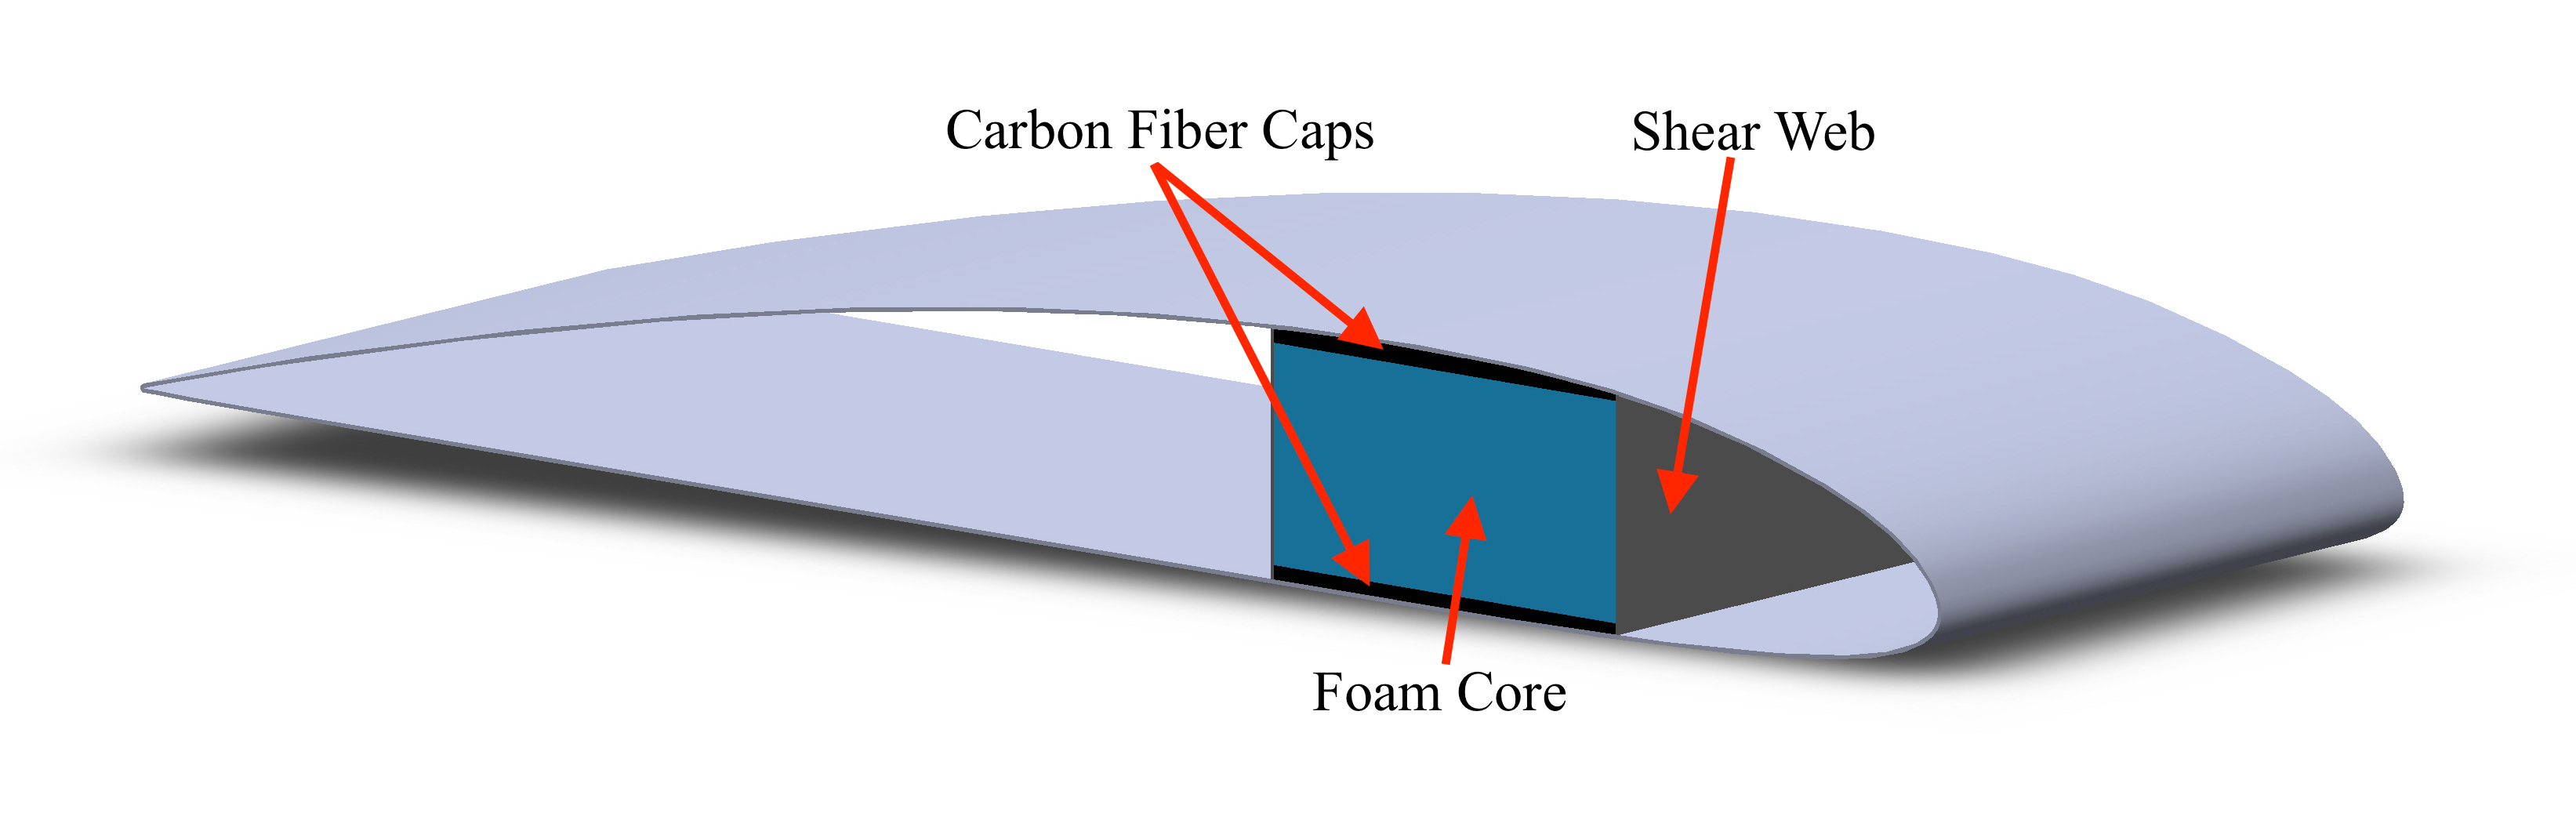
\includegraphics[width=0.6\textwidth]{capspar.pdf}
    \caption{ \textbf{ Cross sectional view of a cap spar.  The two caps are made of carbon fiber, separated by a foam core.}}
	\label{f:capspar}
	\end{center}
\end{figure}

The moment of inertia of the cap spar is modeled by only considering the spar caps, not the foam interior.  
This conservative assumption is made because the contribution of the foam core is much less than that of the spar caps.  
The equation for the moment of inertia\cite{bending} of a cap spar is 

\begin{equation}
    \label{e:moispar}
    I = \frac{w_{\text{cap}}t_{\text{cap}}^3}{6} 2w_{\text{cap}}t_{\text{cap}}\left( \frac{h_{\text{cap}}}{2} + \frac{t_{\text{cap}}}{2} \right)^2
\end{equation}

This equation is not GP compatible.  However, using a first order conservative approximation, the moment of inertia can be expressed as

\begin{equation}
    \label{e:moispar}
    I \leq 2w_{\text{cap}}t_{\text{cap}}\left(\frac{h_{\text{cap}}}{2}\right)^2
\end{equation}

There are also geometric constraints imposed on the width and thickness.  The total spar cap thickness cannot be greater than the thickness of the airfoil cross section, $\tau_t = 0.115$.  The width of the spar cap is assumed by no greater than 30\% of chord, $\tau_w = 0.3$.

\begin{align}
    \label{e:thickness}
    c\tau_t &\geq h_{\text{cap}} + 2t_{\text{cap}} \\
    \label{e:width}
    c\tau_w &\geq w_{\text{cap}} \\
    \end{align}

Generally, a wing is either stress or deflection constrained. Meaning, the wing spar at the root must be strong enough to withstand the bending root moment and stiff enough to not exceed some deflection limit.  Both constraints can be imposed in the optimization model as

\begin{align}
    \label{e:stresscont}
    \sigma_{\text{carbon fiber}} &\geq M_0 \frac{h_{\text{cap}}+t_{\text{cap}}}{I}\\
    \label{e:defcont}
    w_n &\leq \left(\frac{w_{max}}{b/2} \right) b.
\end{align}

The maximum stress for carbon fiber is, $\sigma_{\text{carbon fiber}} = 475$ [MPa]. 
The tip deflection is constrainted to be less than 20\% of the half span, $\frac{w_{max}}{b/2} = 0.2$.

Finally, the weight of the spar cap is computed as

\begin{align}
    \label{e:sparmass}
    \Delta W_i &\geq \rho_{\text{carbon fiber}} w_{\text{cap}_i}t_{\text{cap}_i} \frac{b}{n-1}g \\
    \label{e:sparmasssum}
    W &\geq \sum\limits_{1}^{n-1} \Delta W_i
\end{align}

where $\rho_{\text{carbon fiber}} = 1.4$ [g/cm$^3$].
This cap model is added to the gas-powered long endurance aircraft optimization model and solved by minimizing the max take off weight.  

\subsection{Elliptcal Fuselage for Gas Powered Aircraft}

 
\section{Conclusion}

Using geometric programming as a form of evaluation of the design space, high level intuition and understanding about design trade studies for long-endurance aircraft and their driving requirements is achieved.  
One high level discovery is the important of wind speed.  
If keeping position at all times during the flight is critical to the mission of a proposed aircraft, then that requirement is more likely to be met by a gas-powered architecture.
However, if that constraint can be relaxed such that the aircraft only needs to station keep for 80\% of then time, then for certain latitudes, a solar powered aircraft could achieve greater endurance.
Another unsurprising discovery is the sensitivity of the solar-powered aircraft to the battery energy density and solar cell efficiency.  Using higher energy density batteries can result in significant weight and performance savings.  
The rapid solve time of geometric programming is able to present these trade studies and give intuition into design trades by quantifying the disparity in performance between two options.
While the results of these findings are dependent on the accuracy of the models used in the optimization, it is shown that higher fidelity models can be incorporated to increase accuracy.

\section*{Appendix}

\subsection{Discussion on the use of the \emph{JH01} airfoil}

The \emph{sd7032} airfoil was redesigned to prevent drag creep by weakening the pressure spike associated with premature separation at higher Reynolds numbers.  
Figure~\ref{f:jhcps} shows the a pressure distribution generated in XFOIL of the \emph{JH01} airfoil at $C_L=0.0$ and $C_L=1.35$ with $Re=3e5$.
The redesigned airfoil was named \emph{JH01}. We would like to thank Mark Drela who helped in the redesign.

\begin{figure}[H]
 \begin{subfigmatrix}{2}% number of columns
     \subfigure[$C_L=0.0$\label{f:cpmin}]{\includegraphics{cpmin.pdf}}
     \subfigure[$C_L=1.35$\label{f:cpmax}]{\includegraphics{cpmax.pdf}}
 \end{subfigmatrix}
 \caption{\textbf{ Pressure coefficient plots at the minimum and maximum expected $C_L$ at Reynolds number, $Re=3e5$.  }}
 \label{f:jhcps}
\end{figure}

% produces the bibliography section when processed by BibTeX
\bibliography{biblibrary}
\bibliographystyle{aiaa}

\end{document}

% - Release $Name:  $ -
